% =============================================================================
% MSc thesis defense — "Building Cooperative Robot Behavior from Basic Action Modules"
% Jan M. Straub, Heidelberg University.
% =============================================================================
\documentclass[aspectratio=169,11pt]{beamer}

\usetheme{metropolis}
\metroset{numbering=fraction, progressbar=foot, block=fill}

\usepackage[utf8]{inputenc}
\usepackage[T1]{fontenc}
\usepackage{booktabs}
\usepackage{graphicx}
\usepackage{amsmath}
\usepackage{xcolor}
\usepackage{tikz}

\graphicspath{{images/}}

\definecolor{hdred}{RGB}{198,24,38}
\setbeamercolor{progress bar}{fg=hdred}
\setbeamercolor{title separator}{fg=hdred}
\setbeamercolor{alerted text}{fg=hdred}

% \setbeameroption{show notes on second screen=right}  % enable for dual-screen notes

\title{Building Cooperative Robot Behavior\\from Basic Action Modules}
\subtitle{An LLM-driven control framework for two cooperating AR4 arms}
\author{Jan M.\ Straub\\[0.4em]{\small Supervisor: Prof.\ Dr.\ Artur Andrzejak}}
\institute{Institute for Computer Science --- Artificial Intelligence for Programming\\Ruprecht-Karls-University of Heidelberg}
\date{July 2026}

\begin{document}

% =============================================================================
% OPENING  (~3 min)
% =============================================================================
\maketitle
\note{%
	Welcome. This is my master's thesis on cooperative robot behavior built from basic
	action modules. The one idea I want you to leave with: a small, locally-hosted
	vision-language model, grounded in a structured pool of operations, can drive
	cooperation between two robot arms without fine-tuning and without
	hard-coded sequencing. I'll spend ~30 minutes; please hold questions for the end.}

% --- Overview / outline ------------------------------------------------------
\begin{frame}{Overview}
	\tableofcontents
\end{frame}
\note{%
	A quick map of the talk: I frame the problem, then argue three pillars ---
	grounding for reliability, emergent cooperation, and the narrow boundary ---
	before a short summary and the contributions.}

% --- Slide 2: the answer first (pyramid apex) --------------------------------
\begin{frame}{The answer, up front}
	\begin{block}{Thesis in one sentence}
		A \alert{locally-hosted vision-language model (VLM)}, grounded in a structured pool
		of \alert{29 basic operations}, turns natural language into reliable
		\alert{cooperative dual-arm behavior}, with \alert{no fine-tuning and no
			hard-coded sequencing}.
	\end{block}
	\vfill
	\begin{columns}[t]
		\begin{column}{0.33\textwidth}
			\begin{exampleblock}{Solved}
				\textbf{100\%} success on all single-robot tasks and dual-arm handovers
				(Magistral Small, 25/25 + 5/5 runs).
			\end{exampleblock}
		\end{column}
		\begin{column}{0.33\textwidth}
			\begin{exampleblock}{Emergent}
				Cooperation is reasoned, not scripted. Negotiation lifts dual-robot
				success by \textbf{+25 pp}.
			\end{exampleblock}
		\end{column}
		\begin{column}{0.33\textwidth}
			\begin{alertblock}{One narrow gap}
				Concurrent bimanual lift fails, on \textbf{partner-aware target selection},
				not a missing primitive.
			\end{alertblock}
		\end{column}
	\end{columns}
\end{frame}
\note{%
	I lead with the conclusion deliberately. Three headline claims: single-robot work
	and sequential handoffs are fully solved; coordination emerges from the model's
	reasoning rather than from a script; and there is exactly one task we cannot do yet,
	a simultaneous two-arm lift, and we know precisely why. Everything that follows
	supports these three claims, in this order.}

% --- Slide 3: roadmap --------------------------------------------------------
\begin{frame}{How I'll argue it --- three pillars}
	\begin{enumerate}
		\item[\textbf{1.}] \textbf{Grounding makes it reliable.}\\
		      \small RAG-retrieved operation pool plus reflection give hallucination-free, deterministic plans.
		\item[]\vspace{0.3em}
		\item[\textbf{2.}] \textbf{Cooperation emerges, it is not scripted.}\\
		      \small Signal/wait, parallel groups, and negotiation produce coordination from the prompt alone.
		\item[]\vspace{0.3em}
		\item[\textbf{3.}] \textbf{The boundary is specific and narrow.}\\
		      \small One unsolved task with an identified cause; ablations quantify what each component contributes.
	\end{enumerate}
	\vfill
	\footnotesize First, two minutes on the problem and where this sits in the literature.
\end{frame}
\note{%
	The talk has three pillars matching the three claims. Reliability from grounding,
	emergent cooperation, and an honest account of the boundary. Before the pillars, a
	short problem framing.}

% =============================================================================
% PROBLEM & POSITIONING  (~4 min)
% =============================================================================
\section{The problem}

\begin{frame}{The reasoning--execution gap}
	\begin{columns}[T]
		\begin{column}{0.55\textwidth}
			\small
			\begin{itemize}
				\item Classical robots: precise, but caged. Rigid paths, no tolerance for the unexpected.
				\item VLMs bring world knowledge and reasoning, but cannot reliably turn
				      abstract reasoning into \emph{physical} action.
				\item Models often ignore \alert{past physical state} when planning the next move.
			\end{itemize}
			\begin{block}{Why cooperation is the hard case}
				Two arms must \textbf{avoid collision}, \textbf{share a workspace}, and
				\textbf{synchronize timing}. One prompt decides \emph{which} arm grasps and
				\emph{where} they meet, with no hard-coded sequencing.
			\end{block}
		\end{column}
		\begin{column}{0.45\textwidth}
			\centering
			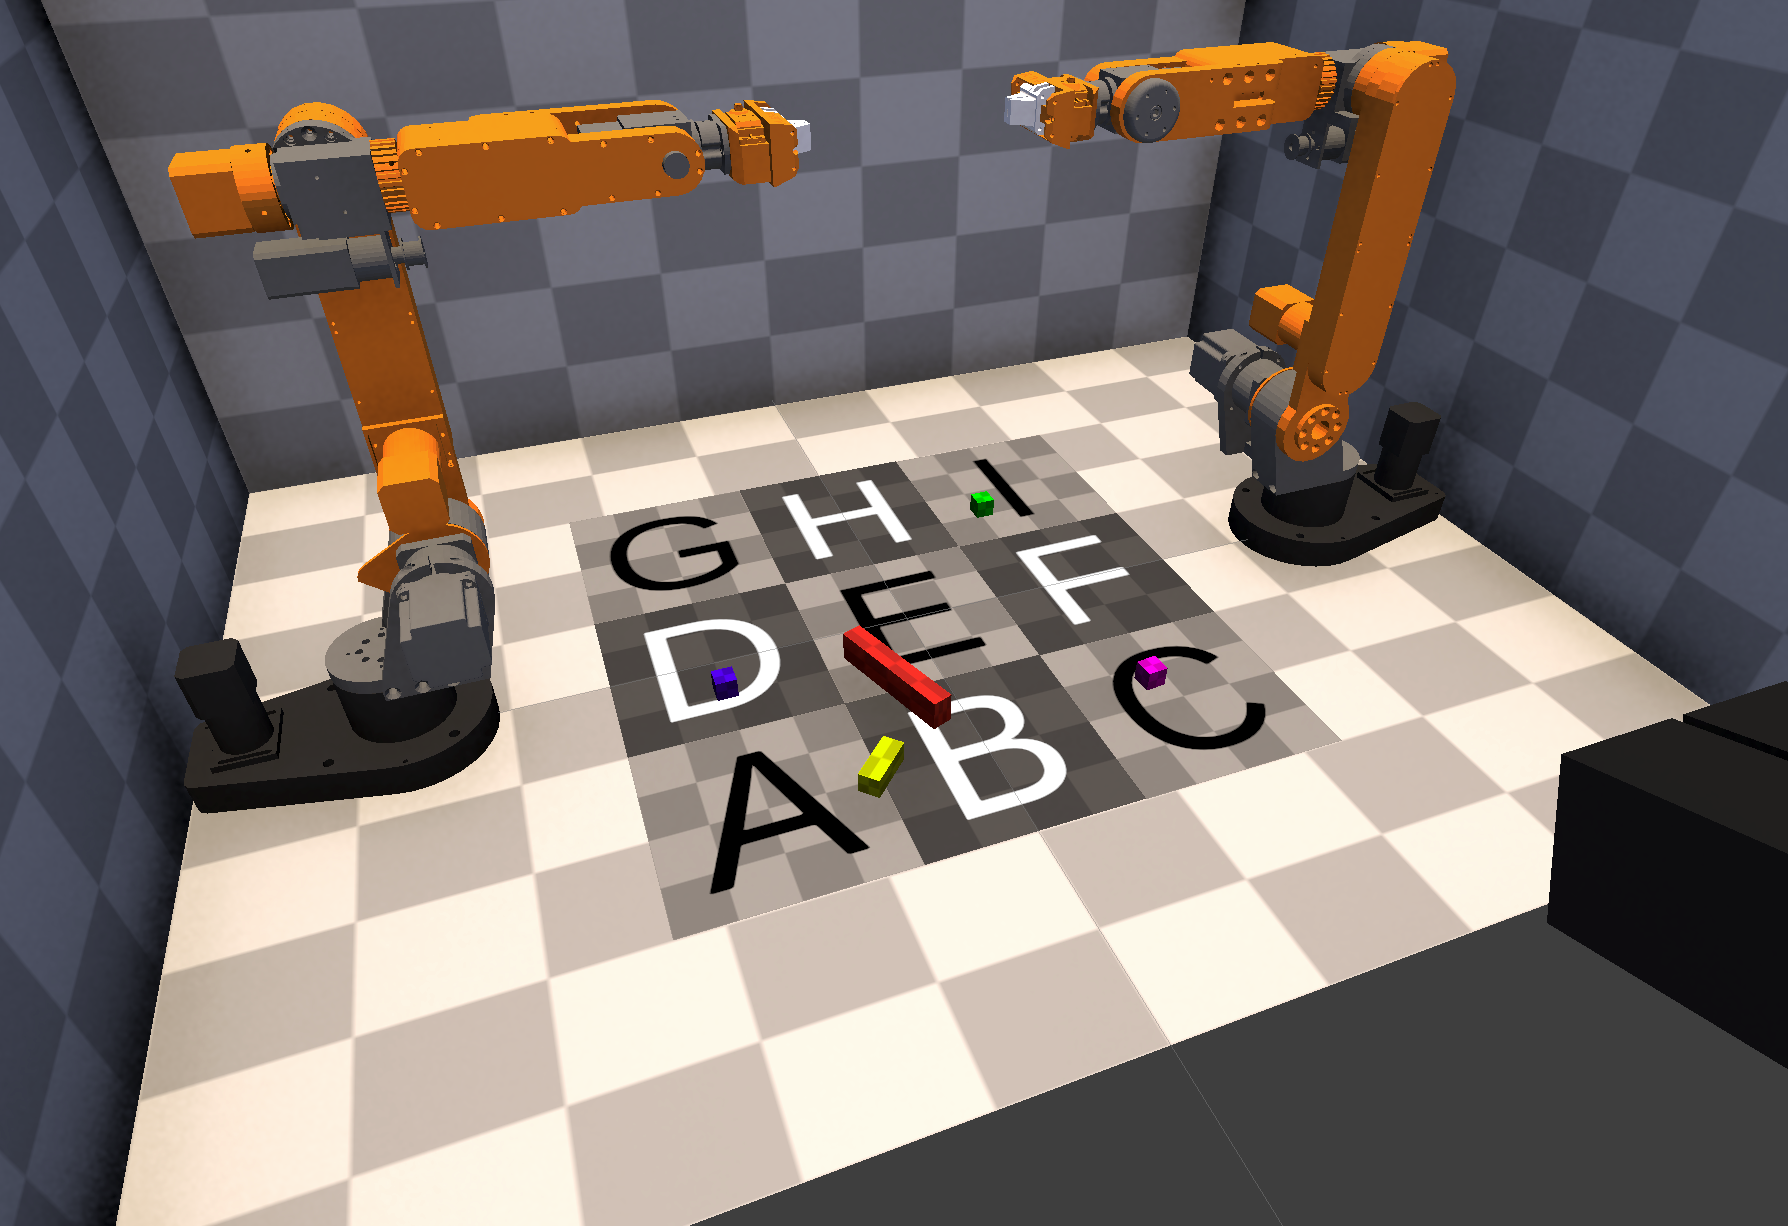
\includegraphics[width=\linewidth,height=0.62\textheight,keepaspectratio]{14_robot_env.png}\\
			\footnotesize Two AR4 arms, a shared workspace, and a stereo camera in Unity.
		\end{column}
	\end{columns}
\end{frame}
\note{%
	Industrial robots are precise but brittle. VLMs reason but don't act reliably ---
	the central gap. Cooperation makes the gap worse: collision avoidance, shared
	workspace, and timing all at once. The high-value tasks --- assembly, handover --- are
	exactly the cooperative ones, which is why I target two arms rather than one.}

\begin{frame}{Two design commitments}
	\begin{columns}[t]
		\begin{column}{0.5\textwidth}
			\begin{block}{Run the model \emph{locally}}
				\begin{itemize}\small
					\item No cloud cost, no external dependency.
					\item No sensitive scene data leaving the machine: data sovereignty.
					\item A compact VLM is enough; we don't need a frontier model.
				\end{itemize}
			\end{block}
		\end{column}
		\begin{column}{0.5\textwidth}
			\begin{block}{Ground the model in \emph{modular operations}}
				\begin{itemize}\small
					\item Reasoning restricted to a vocabulary of \emph{executable} actions.
					\item Separates semantic understanding from physical execution,
					      giving a predictable control rate at the edge.
					\item Vision resolves targets live; no fine-tuning, no task-specific training.
				\end{itemize}
			\end{block}
		\end{column}
	\end{columns}
	\vfill
	\centering\small Backend model: \textbf{Magistral Small 2509 (24B, 4-bit)}: open, EU-origin, vision-capable, runs on a laptop.
\end{frame}
\note{%
	Two commitments. First, local inference --- cost, privacy, and strategic independence;
	and the tasks here don't need a frontier model. Second, ground the model in a modular
	operation pool, which decouples slow semantic reasoning from fast physical control and
	keeps a predictable edge control rate. Backend model is Magistral Small, a 24B open
	model running quantized on a MacBook.}

\begin{frame}{Where this sits --- and the gap it fills}
	\begin{itemize}
		\item \textbf{End-to-end VLA} (RT-2, PaLM-E): great generalization, but data-hungry,
		      opaque, and too slow for the edge.
		\item \textbf{Code-as-Policies}: compositional and transparent, but tied to its API set.
		\item \textbf{Framework-scale} (ROS-LLM, AutoRT): practical scaffolding, but each robot
		      acts on its \emph{own} assignment.
		\item \textbf{RoCo}: per-robot agents negotiate, the direct inspiration for our protocol.
	\end{itemize}
	\vfill
	\begin{alertblock}{Research gap}
		Two arms reasoning \emph{jointly} about a single shared object, cooperation that
		\emph{emerges} from reasoning rather than being engineered from outside, is
		comparatively unexplored.
	\end{alertblock}
\end{frame}
\note{%
	The literature trades generality against reliability. End-to-end models generalize but
	are heavy and opaque; modular code approaches are transparent but API-bound; framework
	systems scale but treat robots independently. RoCo's per-robot negotiation inspired us.
	The open gap: joint reasoning over a shared object, with cooperation emerging
	from reasoning. That is what I set out to build.}

% =============================================================================
% PILLAR 1 — GROUNDING -> RELIABILITY  (~7 min)
% =============================================================================
\section{Pillar 1 --- Grounding makes it reliable}

\begin{frame}{System architecture --- four layers}
	\centering
	
\includegraphics[height=0.78\textheight]{16_system_flow.png}
\end{frame}
\note{%
	Four layers. Layer 1 takes the natural-language command. Layer 2 retrieves relevant
	operations via RAG and the model emits a structured JSON plan. Layer 3 dispatches the
	plan through the sequence executor, handling signal/wait and parallel groups. Layer 4
	executes on the two arms through ROS/MoveIt as a collision-aware planner, or the Unity
	IK pipeline as fallback. The knowledge graph optionally feeds spatial context to
	planning. Built on Unity plus a Python backend plus a Docker ROS2/MoveIt stack.}

\begin{frame}{The vocabulary: a 29-operation registry}
	\begin{columns}[c]
		\begin{column}{0.46\textwidth}
			\footnotesize
			Operations organized by \textbf{complexity}, four tiers:
			\begin{description}\footnotesize
				\item[Atomic (8)] indivisible, no perception: gripper, signal, wait.
				\item[Basic (6)] single dispatch, introduces perception.
				\item[Intermediate (9)] composite; first sees the second robot.
				\item[Complex (6)] full pipelines / tight dual-arm coupling.
			\end{description}
			\vspace{0.4em}
			\textbf{Why tiers?} Failure diagnosis: if a Complex task fails, verify its
			lower-level parts in isolation. The tiers map onto the benchmark difficulty gradient.
		\end{column}
		\begin{column}{0.54\textwidth}
			\centering
			
\includegraphics[width=\linewidth]{09_operation_map.png}
		\end{column}
	\end{columns}
\end{frame}
\note{%
	The model reasons over 29 operations arranged in four complexity tiers, from atomic
	primitives up to full bimanual pipelines. The tiers aren't cosmetic --- they give
	diagnostic value: a failed complex task can be debugged by checking its constituent
	operations in isolation. And the tiers line up with the benchmark difficulty gradient,
	so the evaluation walks up the hierarchy.}

\begin{frame}{The command pipeline --- RAG-grounded planning}
	\centering
	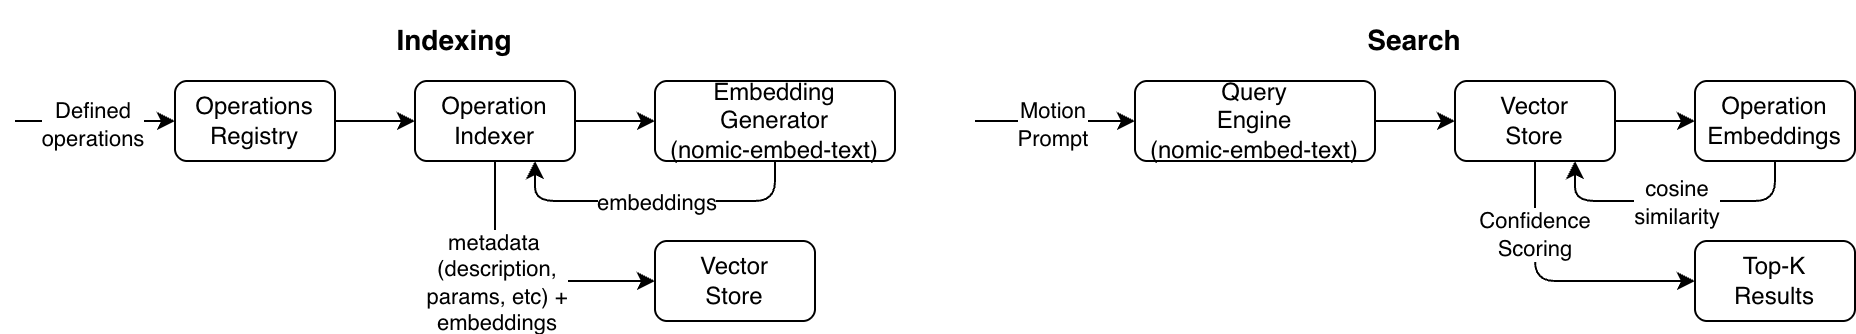
\includegraphics[width=0.92\linewidth]{13_rag.png}
	\vspace{0.3em}
	\begin{columns}[t]
		\begin{column}{0.5\textwidth}\footnotesize
			\textbf{Retrieve, don't enumerate:} embed the instruction, query the operation
			vector store by cosine similarity, inject only the relevant operations and schemas.
		\end{column}
		\begin{column}{0.5\textwidth}\footnotesize
			\textbf{Why it matters:} the model sees only plausible operations.
			Without retrieval, smaller models hallucinated operation names and invalid
			parameters. Variable-passing threads \texttt{detect $\to$ \$target $\to$ move} at runtime.
		\end{column}
	\end{columns}
\end{frame}
\note{%
	The pipeline embeds the instruction, retrieves the most relevant operations, and gives
	the model only those plus their schemas and examples. It returns a JSON plan; the
	sequence executor dispatches step by step and threads outputs into later inputs --- a
	detection result becomes a movement target at runtime. Retrieval narrows the context so
	the model stops inventing non-existent operations, which was a real failure mode early on.}

\begin{frame}{Two more grounding components}
	\begin{columns}[t]
		\begin{column}{0.5\textwidth}
			\begin{block}{Reflection recovery}
				\begin{itemize}\small
					\item On failure, re-query the model with a structured \emph{hint} and recovery
					      suggestions (Reflexion-style verbal feedback).
					\item Closes the perception--action loop at the language level.
					\item Eligibility is gated: no point re-querying a sync barrier.
				\end{itemize}
			\end{block}
		\end{column}
		\begin{column}{0.5\textwidth}
			\begin{block}{Knowledge graph (optional)}
				\begin{itemize}\small
					\item Robots / objects / regions as nodes; reachability, proximity, grasps as edges.
					\item Answers ``who can reach X?'', ``viable handoff?'' via multi-hop queries.
					\item \alert{Spoiler:} measured benefit is \emph{not} positive (Pillar 3).
				\end{itemize}
			\end{block}
		\end{column}
	\end{columns}
\end{frame}
\note{%
	Two more pieces. Reflection: when a step fails, we feed the error and recovery hint back
	to the model for a corrected re-plan --- verbal self-reflection rather than gradient
	updates, gated to failures where a re-plan can actually help. And an optional knowledge
	graph for spatial queries. I flag now that the knowledge graph did not pay off in the
	ablations --- I'll be honest about that in pillar three.}

\begin{frame}{Evidence: grounding $\Rightarrow$ reliability}
	\begin{columns}[c]
		\begin{column}{0.5\textwidth}
			\begin{itemize}\small
				\item \textbf{B1--B5} (navigate $\to$ grasp $\to$ full pick-and-place):
				      \alert{100\% across all 25 runs}, zero hallucinated ops, zero retries.
				\item \emph{Identical} operation sequence on all 5 runs of each benchmark:
				      determinism without prompt engineering.
				\item \textbf{B8} (long chain): 20 sub-tasks, \textbf{85 operations}/run, 5 cycles,
				      all executed, no cascading errors.
			\end{itemize}
			\vspace{0.4em}
			\footnotesize Cost is dominated by \emph{contact-rich} primitives
			(\texttt{grasp\_object}, \texttt{place\_object}), not plan length.
		\end{column}
		\begin{column}{0.5\textwidth}
			\centering
			
\includegraphics[width=\linewidth]{01_success_rate_by_model.png}\\
			\footnotesize Magistral, Ministral, and both Gemma~4 models clear the full single-robot gradient; the Qwen3-VL models break at grasping.
		\end{column}
	\end{columns}
\end{frame}
\note{%
	The evidence for pillar one. Single-robot benchmarks B1 through B5 hit 100% across all
	25 runs with zero hallucinations and zero retries --- and the model emitted the
	identical plan every run, so it's deterministic without prompt tuning. B8 stress-tests
	durability: 85 operations per run across 20 sub-tasks and five cycles, all executed
	cleanly. Time is dominated by physical contact, not by plan length. The figure shows
	only Magistral clears the whole gradient.}

% =============================================================================
% PILLAR 2 — COOPERATION EMERGES  (~7 min)
% =============================================================================
\section{Pillar 2 --- Cooperation emerges}

\begin{frame}{The model composes coordination itself}
	\begin{block}{Two general primitives --- no fixed pattern}
		\begin{itemize}
			\item \texttt{signal} / \texttt{wait\_for\_signal}: one robot pauses at a checkpoint
			      until the other signals readiness.
			\item \textbf{Parallel groups}: operations dispatched concurrently when no ordering is needed.
		\end{itemize}
	\end{block}
	\vfill
	The executor imposes \alert{no} coordination policy. The model decides \emph{where}
	synchronization is needed and \emph{which} steps can run in parallel, guided only by
	general rules in the prompt, never an explicit script.
	\vfill
	\footnotesize The low-level control layer is unaware any coordination is happening.
\end{frame}
\note{%
	Coordination is built from just two general primitives: a signal/wait pair and parallel
	groups. Crucially the executor enforces no coordination pattern of its own --- the model
	composes these primitives, deciding where to synchronize and what to parallelize. The
	control layer below doesn't even know coordination is happening. That's what makes the
	next results "emergent".}

\begin{frame}{B6 --- the handoff, solved}
	\begin{columns}[c]
		\begin{column}{0.5\textwidth}
			\footnotesize
			Prompt: \emph{``Robot1 grasps the red cube and hands it to Robot2.''}
			\vspace{0.4em}
			\begin{itemize}
				\item Magistral: \alert{100\%} success, 5/5 runs; 47/47 operations succeed first try.
				\item 4/5 runs: the \emph{identical} 9-operation plan.
				\item The model \textbf{inserts a synchronization barrier} so Robot2 receives only
				      after Robot1 signals, \alert{never stated in the prompt}.
				\item Ministral also solves it (100\%); Gemma-4B partial (3/5); the Qwen3 models and Gemma-2B break down at plan construction.
			\end{itemize}
		\end{column}
		\begin{column}{0.5\textwidth}
			\centering
			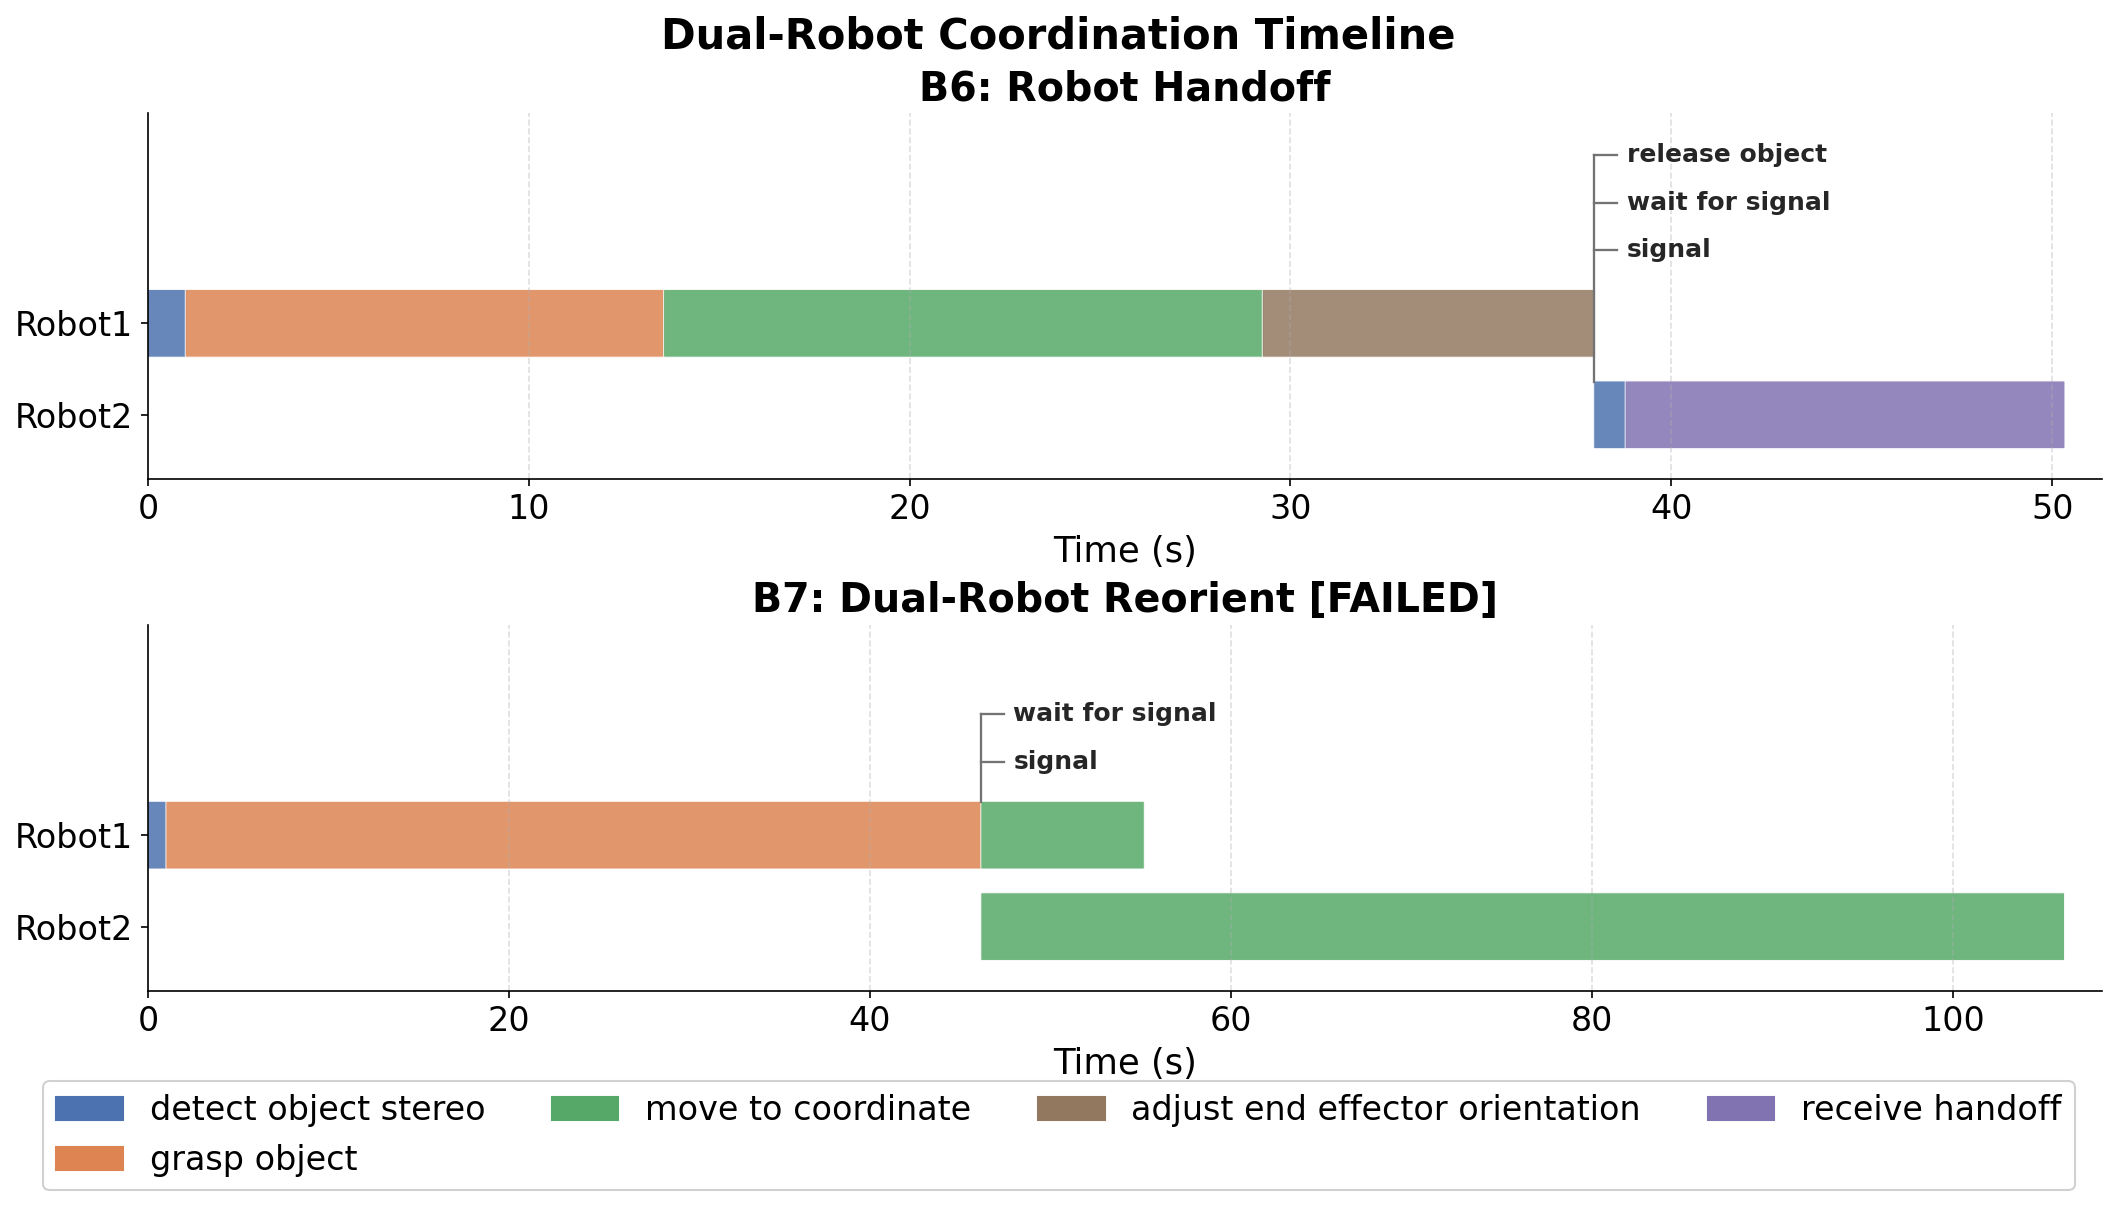
\includegraphics[width=\linewidth]{07_coordination_timeline.png}\\
			\footnotesize Top: successful handoff. Bottom: the B7 failure (Pillar 3).
		\end{column}
	\end{columns}
\end{frame}
\note{%
	B6 is the headline cooperation result. From a single sentence, Magistral produces a
	nine-operation handoff plan, 100\% success, and inserts the synchronization barrier
	itself so the receiver waits for the giver --- temporal dependency the prompt never
	spells out. Magistral and Ministral both solve it; Gemma-4B succeeds in three of five runs;
	the Qwen models and Gemma-2B fail earlier in planning. The top
	timeline shows the clean handoff.}

\begin{frame}{B10 --- emergent parallelism}
	\footnotesize Prompt: two robots, two \emph{disjoint} pick-and-place tasks, no shared resources.
	\vspace{0.5em}
	\begin{itemize}
		\item \alert{100\%} success, 40/40 operations, zero retries.
		\item Model recognized independence \emph{unprompted} and emitted a
		      \textbf{parallelism ratio of 0.75}, identical across all 5 runs.
		\item Heavy manipulation phases run concurrently; detection kept sequential, a
		      conservative, stable choice.
	\end{itemize}
	\vfill
	\begin{exampleblock}{Takeaway}
		The model expresses physical simultaneity when the task allows it,
		the same capability that matters for the unsolved B7.
	\end{exampleblock}
\end{frame}
\note{%
	B10 shows the other side of coordination: parallelism. Two independent pick-and-place
	tasks. The model recognized they were independent without being told, and parallelized
	the heavy manipulation while keeping detection sequential --- a 0.75 parallelism ratio,
	identical every run. Remember this: the model CAN schedule simultaneous action. That
	matters when we get to B7.}

\begin{frame}{Negotiation --- distributing the reasoning}
	\begin{columns}[T]
		\begin{column}{0.55\textwidth}
			\footnotesize
			A single model planning for both arms under-specifies roles and emits
			\emph{implicit conflicts} that surface only at execution.
			\vspace{0.4em}

			\textbf{Protocol} (central hub, up to 3 rounds):
			\begin{enumerate}
				\item \textbf{Analyze}: each robot's agent assesses its own role (parallel).
				\item \textbf{Propose}: one agent per round drafts a \emph{complete} plan (round-robin).
				\item \textbf{Evaluate}: peers accept/reject with justification; \alert{unanimity} required.
			\end{enumerate}
			\vspace{0.3em}
			No consensus after 3 rounds, fall back to single-model parsing.
		\end{column}
		\begin{column}{0.45\textwidth}
			\begin{block}{Design intent}
				\footnotesize Surface disagreements \emph{as language}, before they become
				collisions. Inspired by RoCo; each robot reasons from its own perspective.
			\end{block}
		\end{column}
	\end{columns}
\end{frame}
\note{%
	For role-ambiguous tasks we distribute reasoning. Each robot gets its own agent. Three
	phases run through a central hub: analyze in parallel, then one agent proposes a complete
	plan per round in round-robin, then peers evaluate and must unanimously accept. Up to
	three rounds, then fall back to single-model parsing. The point, following RoCo, is to
	make conflicts appear as language rather than as collisions.}

\begin{frame}{B13 --- negotiation pays off}
	\begin{columns}[c]
		\begin{column}{0.52\textwidth}
			\begin{table}\footnotesize
				\begin{tabular}{lcc}
					\toprule
					                        & \textbf{Task SR}     & \textbf{Ops/run} \\
					\midrule
					Negotiation \textbf{on} & \alert{0.80} (16/20) & 35.2             \\
					Negotiation off         & 0.55 (11/20)         & 26.2             \\
					\bottomrule
				\end{tabular}
			\end{table}
			\vspace{0.4em}
			\footnotesize
			\begin{itemize}
				\item \alert{+25 pp} task success; no enabled run dropped below 3/4 tasks.
				\item Without it, 4/5 runs lost \emph{half} their tasks to collision/role conflicts.
				\item Negotiation \emph{halves} conflict incidence and \emph{confines} the damage.
				\item Cost is \textbf{front-loaded} (~2 rounds), not per-step.
			\end{itemize}
		\end{column}
		\begin{column}{0.48\textwidth}
			\centering
			
\includegraphics[width=\linewidth]{08_ablation.png}\\
			\footnotesize Per-component ablation deltas (Magistral, $n=5$).
		\end{column}
	\end{columns}
\end{frame}
\note{%
	And the ablation confirms it: negotiation raises dual-robot task success from 0.55 to
	0.80, +25 points --- the single largest effect among all components. Without it, four of
	five runs lost half their tasks to collision and role conflicts. Negotiation doesn't
	eliminate conflicts but roughly halves them and contains the fallout, and its cost is a
	fixed front-loaded couple of rounds, not a per-step penalty.}

% =============================================================================
% PILLAR 3 — THE BOUNDARY  (~6 min)
% =============================================================================
\section{Pillar 3 --- The boundary is narrow and specific}

\begin{frame}{B7 --- concurrent bimanual lift: the one we can't do}
	\footnotesize Task: Robot1 grasps to stabilize, Robot2 grasps the opposite side, \emph{both lift together}.
	\vspace{0.3em}
	\begin{columns}[T]
		\begin{column}{0.5\textwidth}
			\textbf{0\% task success, all six models.} Two failure modes:
			\begin{enumerate}\footnotesize
				\item \texttt{wait\_for\_signal} never dispatched once control crosses robots
				      outside a \texttt{parallel\_group} (3/5 runs).
				\item Final lift: two \emph{independently} chosen targets land $\sim$0.10\,m apart,
				      violating the 0.2\,m separation check (2/5 runs).
			\end{enumerate}
		\end{column}
		\begin{column}{0.5\textwidth}
			\begin{alertblock}{The gap is NOT a missing primitive}
				\footnotesize
				\texttt{synchronized\_grasp} / \texttt{stabilize\_object} exist, and the task
				doesn't even need them. What's missing: \alert{partner-aware target selection}.
				Each arm picks a valid target; nothing checks one \emph{against the other}.
			\end{alertblock}
			\footnotesize\vspace{0.3em}
			Deeper sim limit: a Unity \texttt{Transform} has one parent, so a single object
			can't attach to two grippers at once.
		\end{column}
	\end{columns}
\end{frame}
\note{%
	Now the boundary. B7 asks both arms to lift one shared object together. Every model
	fails. Two modes: a cross-robot wait that's never dispatched outside a parallel group,
	and a final lift where each arm picks an individually valid target but the two land too
	close. The key diagnosis: this is NOT a missing operation --- the bimanual primitives
	exist and the task doesn't even require them. The missing capability is partner-aware
	target selection: nothing checks one arm's target against the other's. There's also a
	simulation limit --- a Unity Transform has one parent, so true co-grasp needs a shared
	attachment model.}

\begin{frame}{Honest ablation synthesis --- what each piece really does}
	\begin{table}\footnotesize
		\begin{tabular}{lll}
			\toprule
			\textbf{Component}    & \textbf{Effect}     & \textbf{Reading}                                                  \\
			\midrule
			Negotiation (B13)     & \alert{+25 pp}      & Genuine reliability gain                                          \\
			ROS/MoveIt (B16)      & +24 pp\,$^\dagger$  & $^\dagger$gap is a shared detection flake;                        \\
			                      &                     & \quad value is \emph{capability} (collision-aware)                \\
			Reflection (B12)      & +16 pp (task)       & Clears transient motion failures; +6 pp at op level               \\
			RAG (B11)             & model-dependent     & Helps Gemma, \alert{hurts} Qwen3, neutral for Magistral/Ministral \\
			Knowledge graph (B14) & small \emph{cost}   & Prompt over-anchoring, not a broken component                     \\
			VGN grasp (B15)       & \alert{+35 pp} Magi & 6-DOF pose orients gripper to angled objects;                     \\
			                      & (+33 pp pooled)     & \quad scored on held-and-lifted, all 6 models                     \\
			\bottomrule
		\end{tabular}
	\end{table}
	\vfill
	\begin{alertblock}{Caveat (stated up front)}
		\footnotesize Task/grasp deltas are point estimates at \textbf{$n=5$} per condition,
		one simulated environment (VGN pooled is $n=30$ across six models). Enough to expose
		deterministic failure modes; not enough to separate effects within one standard
		deviation. Read them as a range.
	\end{alertblock}
\end{frame}
\note{%
	Being honest about the ablations. Negotiation is a real +25. ROS/MoveIt looks like +24
	but that gap is actually a shared stereo-detection flake --- its real value is
	capability, collision-aware planning, not measured reliability. Reflection is +16 at the
	task level, +6 at the operation level. RAG is model-dependent: it helps Gemma, hurts
	Qwen3, neutral for Magistral and Ministral --- so enable it per model. The knowledge graph carries a
	small cost from prompt over-anchoring. VGN is a real +35 for Magistral (70 vs 35 percent
	held-and-lifted), +33 pooled across all six models, once you score grasps on whether the
	object is actually held and lifted, not just the gripper-close ack. Its 6-DOF pose
	orients the gripper to angled objects the top-down baseline closes on but drops, and it's
	the one positive effect that holds for all six models. And the honesty caveat: n=5, one
	environment --- treat deltas as ranges, not exact figures.}

\begin{frame}{AutoRT adaptation \& the safety gate (B17)}
	\begin{columns}[c]
		\begin{column}{0.52\textwidth}
			\footnotesize
			Re-targeted AutoRT for \emph{fixed-base} manipulation: observe $\to$ generate $\to$
			filter $\to$ select, dropping locomotion, with a structured object manifest instead
			of raw images.
			\vspace{0.4em}

			\textbf{Two-layer safety (Robot Constitution):}
			\begin{itemize}
				\item Semantic VLM check (temp 0), plus
				\item \alert{Hard kinematic check} the semantic layer can't override (bounds, velocity, separation).
			\end{itemize}
			\vspace{0.3em}
			Result: \alert{false-accept rate 0.0}, never admits an unsafe task; reproducible
			confusion matrix every run. Slightly over-rejects aggressive-but-safe phrasing (FR 0.25).
		\end{column}
		\begin{column}{0.48\textwidth}
			\centering
			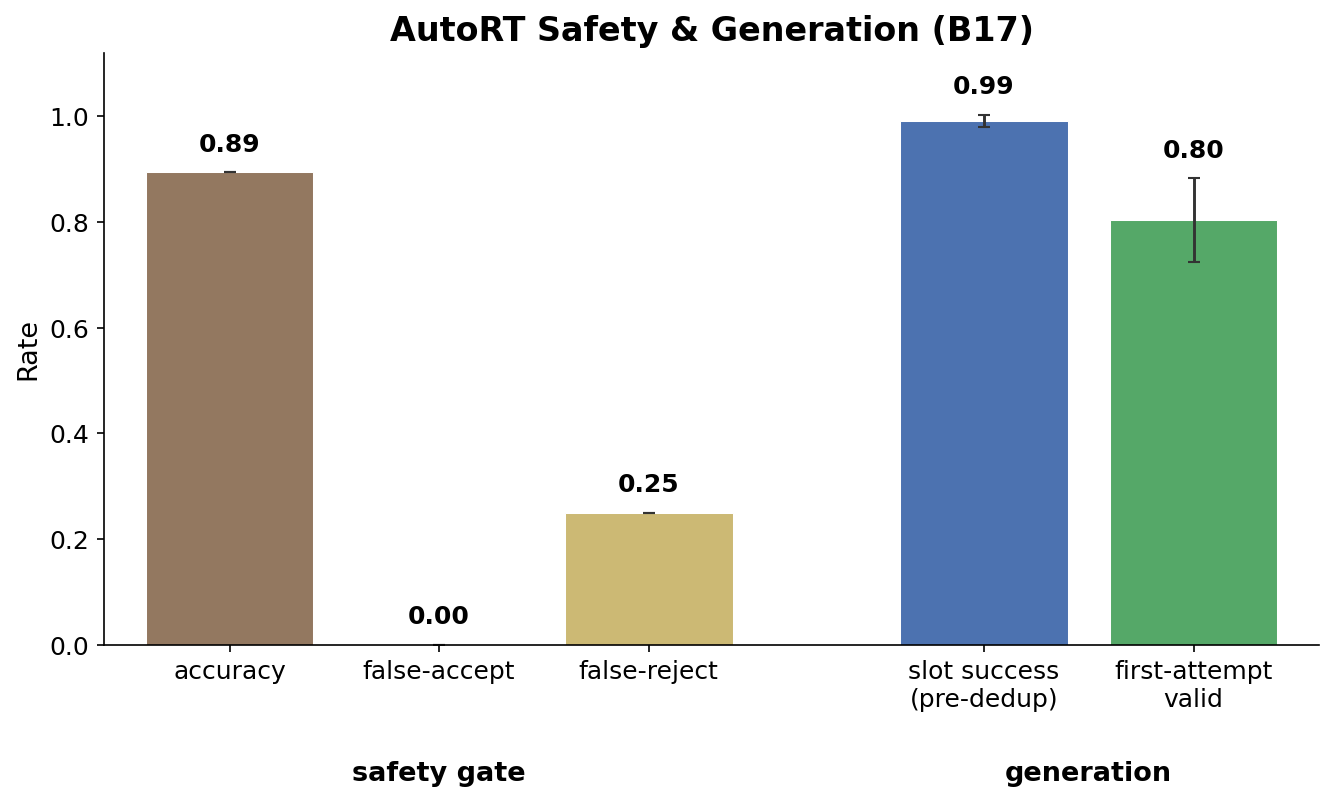
\includegraphics[width=\linewidth]{10_autort_safety.png}
		\end{column}
	\end{columns}
\end{frame}
\note{%
	The fourth contribution: an AutoRT adaptation for our fixed-base setting. The loop
	observes, generates two candidate tasks, filters, and selects. The safety filter is two
	layers --- a semantic VLM check plus a hard kinematic code check that the model cannot
	override. The gate is conservative by design: zero false accepts across all runs, fully
	reproducible at temperature zero. It does over-reject about a quarter of aggressively
	phrased but safe tasks, which sits in the semantic layer, not the kinematic guarantees.}

\begin{frame}{Limitations --- the real blockers}
	\begin{columns}[t]
		\begin{column}{0.5\textwidth}
			\begin{block}{Sensing}
				\footnotesize Stereo depth degrades on textureless surfaces ($\sim$1.8$\times$ scale bias),
				so VGN is unreliable and we fell back to geometric. No force-torque feedback.
			\end{block}
			\begin{block}{Latency}
				\footnotesize VLM parse $\approx$ \textbf{18\,s} median, which precludes \emph{reactive} control;
				re-plan only between motions, never during.
			\end{block}
		\end{column}
		\begin{column}{0.5\textwidth}
			\begin{block}{Sim-to-real}
				\footnotesize PD gains, compliance, backlash, grasp-force thresholds all tuned for
				simulation, so they need revalidation on hardware.
			\end{block}
			\begin{block}{Validation \& scope}
				\footnotesize 4/6 models forward impossible inputs (B9); the guard belongs downstream
				or pre-parse. Everything is $n=5$, one sim environment.
			\end{block}
		\end{column}
	\end{columns}
\end{frame}
\note{%
	The honest limitations. Sensing is the big one: stereo depth is too noisy on synthetic
	surfaces for VGN, so we fall back to a geometric planner, and there's no force-torque
	feedback. Latency: an 18-second median parse rules out reactive control --- we re-plan
	between motions, not during. Sim-to-real: gains and thresholds are simulation-tuned. And
	validation: four of six models don't reject impossible instructions at parse time, so
	that guard needs to move downstream or pre-parse; plus the n=5 caveat throughout.}

% =============================================================================
% SUMMARY  (~1 min)
% =============================================================================
\section{Summary}

\begin{frame}{Summary --- results at a glance}
	\begin{columns}[T]
		\begin{column}{0.5\textwidth}
			\footnotesize
			\textbf{What works}
			\begin{itemize}\footnotesize
				\item Single-robot B1--B5: \alert{100\%}, 25/25 runs, deterministic plans.
				\item Long chain B8: 85 ops/run, 5 cycles, no cascading errors.
				\item Handoff B6: \alert{100\%}, self-inserted sync barrier.
				\item Parallelism B10: 0.75 ratio, recognized unprompted.
				\item Safety gate B17: false-accept \alert{0.0}, reproducible.
			\end{itemize}
		\end{column}
		\begin{column}{0.5\textwidth}
			\footnotesize
			\textbf{What each component contributes}
			\begin{itemize}\footnotesize
				\item Negotiation (B13): \alert{+25 pp} task success.
				\item VGN grasp (B15): \alert{+35 pp} Magistral, +33 pp pooled.
				\item Reflection (B12): +16 pp task.
				\item RAG (B11): model-dependent; KG (B14): small cost.
			\end{itemize}
			\vspace{0.5em}
			\textbf{The one open gap}
			\begin{itemize}\footnotesize
				\item Concurrent bimanual B7: \alert{0\%}, all six models.
				\item Cause: \alert{partner-aware target selection}, not a missing primitive.
			\end{itemize}
		\end{column}
	\end{columns}
	\vfill
	\footnotesize All deltas are $n=5$ point estimates in one sim environment (VGN pooled $n=30$); read as ranges.
\end{frame}
\note{%
	One slide to consolidate before the contributions. Left, what works: the full
	single-robot gradient, the long-chain durability test, the handoff with its
	self-inserted barrier, emergent parallelism, and the conservative safety gate. Middle/
	right, the component contributions, ranked within their outcome axis: negotiation and
	VGN are the largest, reflection moderate, RAG model-dependent, knowledge graph a small
	cost. And the single open gap, B7, with its named cause. The caveat on sample size
	carries through all of it.}

% =============================================================================
% CLOSE  (~3 min)
% =============================================================================
\section{Conclusion}

\begin{frame}{Four contributions}
	\begin{enumerate}
		\item \textbf{LLM orchestration layer}: local VLM, RAG retrieval, two-phase
		      chain-of-thought, runtime variable-passing. No hard-coded sequences, no fine-tuning.
		\item \textbf{Hierarchical 29-operation registry}: four tiers; doubles as the
		      reasoning vocabulary \emph{and} a failure-diagnosis tool.
		\item \textbf{Dual-arm negotiation protocol}: per-robot agents, analyze/propose/evaluate;
		      +25 pp on role-ambiguous tasks.
		\item \textbf{AutoRT adaptation}: fixed-base task generation plus a two-layer Robot
		      Constitution with hard kinematic guarantees.
	\end{enumerate}
\end{frame}
\note{%
	To summarize, four contributions: the orchestration layer that needs no fine-tuning; the
	hierarchical operation registry that doubles as a diagnosis tool; the negotiation
	protocol worth +25 points; and the AutoRT adaptation with hard safety guarantees.}

\begin{frame}{Path to a real robot --- a config change, not a rewrite}
	\begin{itemize}
		\item Hardware abstraction boundary: \texttt{--env real} swaps camera and hardware adapters,
		      \alert{zero operation-code changes}.
		\item Default \textbf{hybrid} control: ROS/MoveIt collision-aware planning, Unity fallback,
		      the correct route for physical AR4 hardware, already dual-robot configured.
	\end{itemize}
	\vfill
	\begin{block}{Two remaining blockers}
		\footnotesize
		\textbf{Depth sensing}: a RealSense/ToF source behind the existing
		\texttt{get\_depth\_frame} stub releases the VGN pipeline unchanged.\\
		\textbf{Force-torque feedback}: a wrist sensor replaces the contact-duration heuristic.
	\end{block}
\end{frame}
\note{%
	The architecture is deliberately ready for hardware: a single flag swaps to the real
	adapters with no operation-code changes, and the default hybrid mode already uses the
	ROS/MoveIt path that physical AR4 hardware needs. Two blockers remain, both hardware: a
	real depth sensor behind an existing stub, and a force-torque sensor to replace the
	contact heuristic.}

\begin{frame}{Future work}
	\begin{itemize}
		\item \textbf{Depth upgrade}: an active-stereo / ToF sensor fully releases VGN-grade grasping.
		\item \textbf{Bimanual pre-pass}: detect ``simultaneous grasp'' language, route to a
		      bimanual-aware prompt; directly attacks the B7 gap.
		\item \textbf{Pre-parse validation}: robot-ID and object-existence checks before any
		      model call (closes B9 deterministically).
		\item \textbf{Faster inference}: distilled task-specific models plus speculative parsing to
		      shrink the 18\,s window.
	\end{itemize}
\end{frame}
\note{%
	Future work follows from the limitations: a real depth sensor; a bimanual pre-pass that
	detects simultaneous-grasp language and surfaces the right primitive, attacking B7;
	pre-parse validation to deterministically reject impossible inputs; and faster inference
	via distillation and speculative parsing.}

\begin{frame}[standout]{The answer, restated}
	Single-robot manipulation and sequential dual-arm coordination: \textbf{solved}.\\[0.5em]
	Cooperation: \textbf{emergent}, composed by the model, not scripted.\\[0.5em]
	Concurrent bimanual: \textbf{not yet}, gap is narrow and named:\\
	\alert{partner-aware target selection}.\\[0.8em]
	\footnotesize A foundation model \emph{can} coordinate cooperation between two arms
	by decomposing language into basic operations.
\end{frame}
\note{%
	To close, the apex restated. Single-robot and sequential cooperation are solved.
	Cooperation is emergent, composed by the model. The one unsolved task fails on a narrow,
	named gap --- partner-aware target selection --- and notably the model already expresses
	simultaneity (B10), it just can't yet choose mutually compatible targets. The central
	claim holds: a foundation model can coordinate cooperation from a vocabulary of
	basic operations.}

\begin{frame}[standout]{Thank you}
	\centering
	Questions?
	\vfill
	\footnotesize Jan M.\ Straub --- \texttt{github.com/JanMStraub/Cooperative-Robot-Behavior-from-Basic-Action-Modules}
\end{frame}
\note{Thank you --- happy to take questions. Backup slides follow for B7 detail, latencies, and the model--task matrix.}

% =============================================================================
% BACKUP
% =============================================================================
\appendix

\begin{frame}{Backup --- B7 per-run outcomes}
	\begin{table}\footnotesize
		\begin{tabular}{ccll}
			\toprule
			\textbf{Run} & \textbf{Ops ok} & \textbf{Dur (s)} & \textbf{Failing op}                       \\
			\midrule
			1            & 4/8             & 111              & \texttt{wait\_for\_signal}                \\
			2            & 4/10            & 43               & \texttt{wait\_for\_signal}                \\
			3            & 6/7             & 211              & \texttt{move\_to\_coordinate} (collision) \\
			4            & 6/7             & 206              & \texttt{move\_to\_coordinate} (collision) \\
			5            & 4/10            & 46               & \texttt{wait\_for\_signal}                \\
			\bottomrule
		\end{tabular}
	\end{table}
	\footnotesize Two clusters: synchronization deadlock (1,2,5) and lift-target collision at $\sim$0.10\,m (3,4).
\end{frame}
\note{B7 detail: three runs deadlock at the cross-robot wait, two reach the lift and collide at ~0.10 m.}

\begin{frame}{Backup --- single-robot operation latencies}
	\begin{table}\footnotesize
		\begin{tabular}{llcc}
			\toprule
			\textbf{Operation}              & \textbf{Bench} & \textbf{n} & \textbf{Mean (s)} \\
			\midrule
			\texttt{detect\_object\_stereo} & B1--B5         & 30         & 0.80              \\
			\texttt{move\_to\_coordinate}   & B1--B3         & 20         & 4.37              \\
			\texttt{grasp\_object} (B3)     & B3             & 5          & 19.84             \\
			\texttt{grasp\_object} (B4)     & B4             & 5          & 10.93             \\
			\texttt{place\_object}          & B4             & 5          & 34.43             \\
			\bottomrule
		\end{tabular}
	\end{table}
	\footnotesize Perception is cheap and stable; contact-rich manipulation dominates and varies with object pose.
\end{frame}
\note{Latency backup: perception under a second; grasp and place dominate and depend on object pose.}

\begin{frame}{Backup --- model $\times$ task matrix}
	\centering
	
\includegraphics[height=0.8\textheight]{02_model_task_heatmap.png}
\end{frame}
\note{Full model-by-task matrix. Note B9: only Qwen-30B and Gemma-2B correctly refuse the impossible task --- the inverted ordering, and it doesn't track model scale.}

\end{document}
